\section{Testbench bitcell}
\textit{Testbench for your chosen bitcell, where you have simulated it’s functionality on structural level using only Boolean gates and interconnect using Verilog and ActiveHDL.}

Here is the testbench we used for the bitcell:

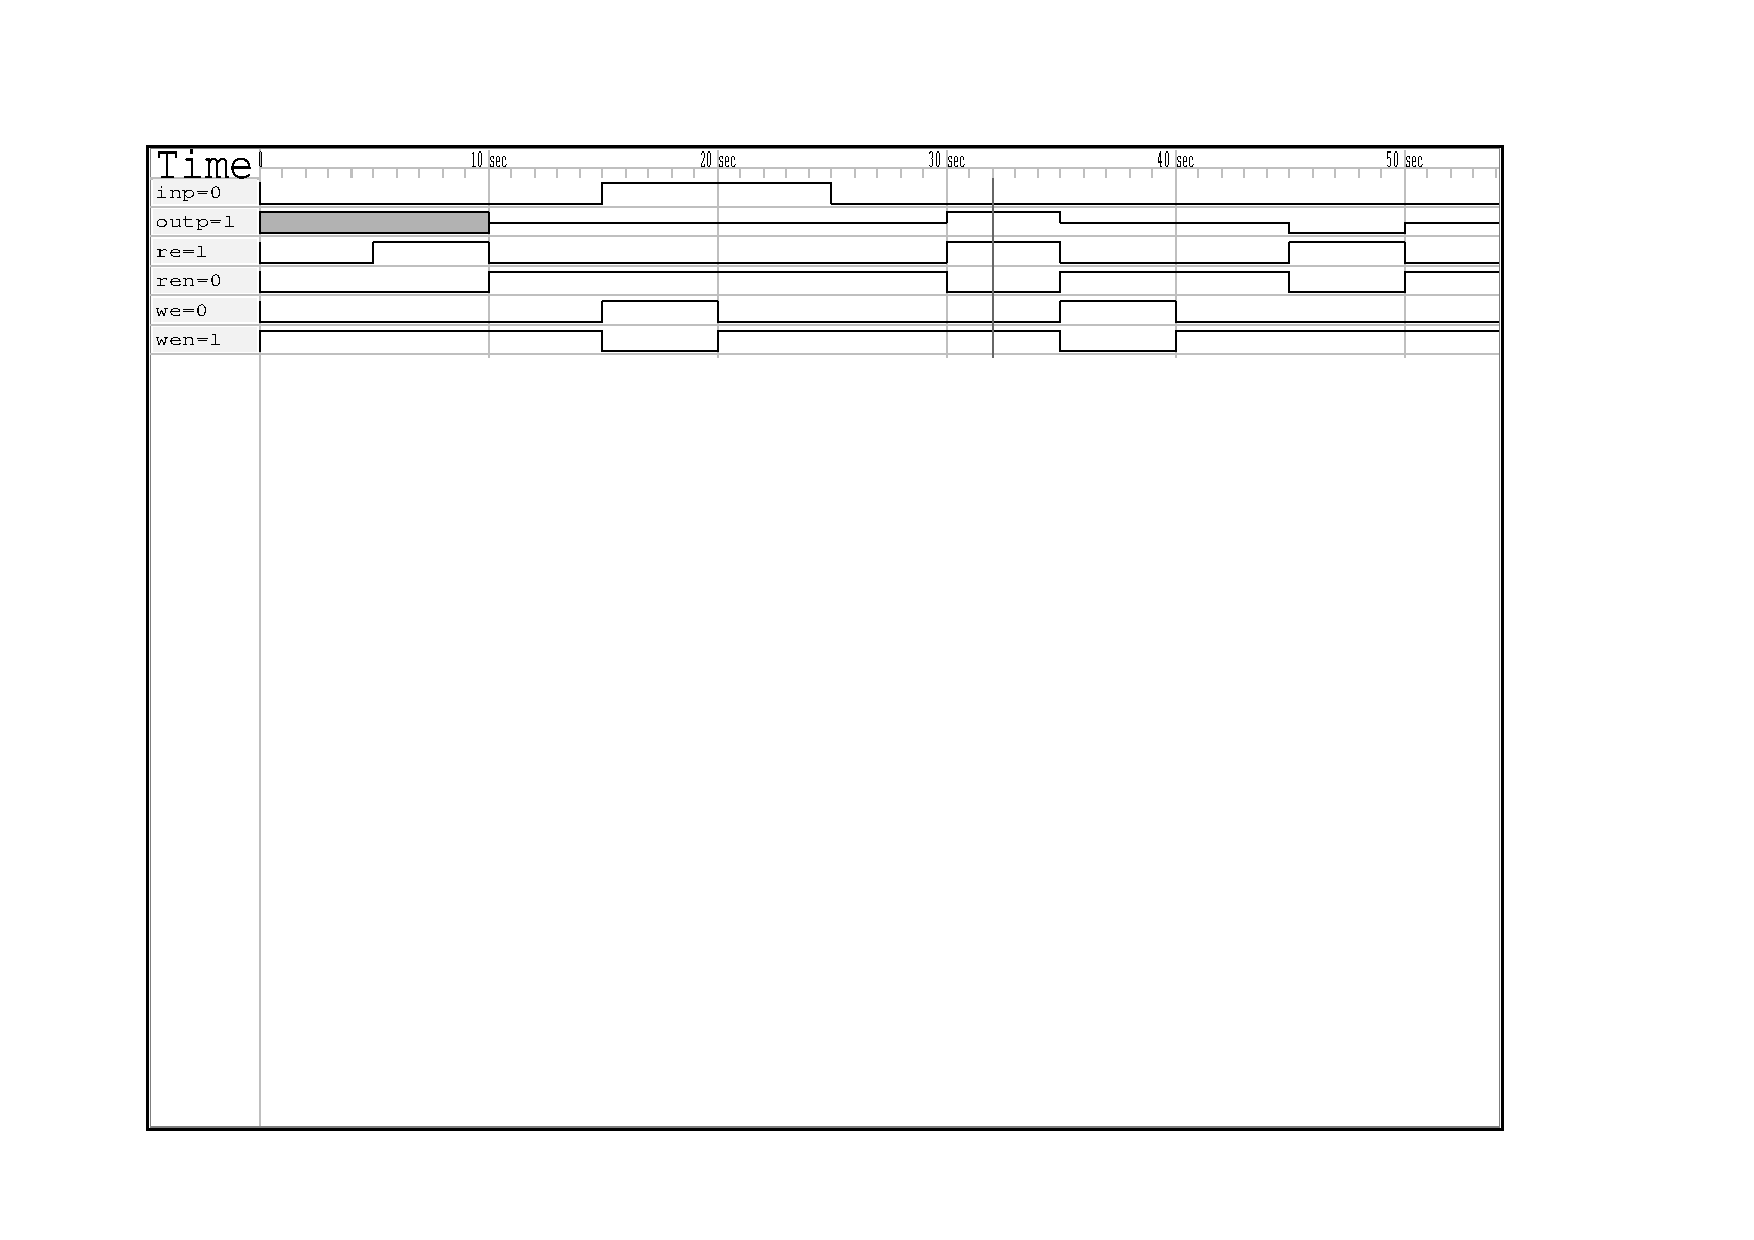
\includegraphics[width=\textwidth]{verilog_mem8x8_latch/simple_testbenches/bitcell.pdf}

We designed our bitcell like the latch with two NOT gates feeding each others output to the others input that was introduced in the lecture Wednesday 16/10. We made sure to include transmission gates on the input, on the backpropagation and on the output. Thus the output is high resistance when not reading, and we don't need any MUX to choose which byte to read or anything like that, but just read from a shared databus.

That means we strayed somewhat from the design specifications, which say they would like only 4 inputs, but we desided that taking these inputs would reduce the total amount of transistors needed, since inverting control signals could be shared between all bitcells.

We have implemented it all in Verilog (not System Verilog) in VSCode, and compiled with Icarus Verilog.